%% 
%% Copyright 2019-2021 Elsevier Ltd
%% 
%% This file is part of the 'CAS Bundle'.
%% --------------------------------------
%% 
%% It may be distributed under the conditions of the LaTeX Project Public
%% License, either version 1.2 of this license or (at your option) any
%% later version.  The latest version of this license is in
%%    http://www.latex-project.org/lppl.txt
%% and version 1.2 or later is part of all distributions of LaTeX
%% version 1999/12/01 or later.
%% 
%% The list of all files belonging to the 'CAS Bundle' is
%% given in the file `manifest.txt'.
%% 
%% Template article for cas-dc documentclass for 
%% double column output.

\documentclass[a4paper,fleqn]{cas-dc}

% If the frontmatter runs over more than one page
% use the longmktitle option.

%\documentclass[a4paper,fleqn,longmktitle]{cas-dc}

\usepackage[numbers]{natbib}
%\usepackage[authoryear]{natbib}
%\usepackage[authoryear,longnamesfirst]{natbib}

%%%Author macros
\def\tsc#1{\csdef{#1}{\textsc{\lowercase{#1}}\xspace}}
\tsc{WGM}
\tsc{QE}
%%%

% Uncomment and use as if needed
\newtheorem{theorem}{Algorithm}
\newtheorem{lemma}[theorem]{Lemma}
%\newdefinition{rmk}{Remark}
%\newproof{pf}{Proof}
%\newproof{pot}{Proof of Theorem \ref{thm}}

\begin{document}
\let\WriteBookmarks\relax
\def\floatpagepagefraction{1}
\def\textpagefraction{.001}

% Short title
%\shorttitle{<short title of the paper for running head>}    

% Short author
\shortauthors{B.T. Rawlins et el.}  

% Main title of the paper
\title [mode = title]{Validation of an integrated data-driven surrogate model and a thermo-hydraulic network based model to determine boiler operational loads using a fully connected mixture density network}  

% Title footnote mark
% eg: \tnotemark[1]
%\tnotemark[<tnote number>] 

% Title footnote 1.
% eg: \tnotetext[1]{Title footnote text}
%\tnotetext[<tnote number>]{<tnote text>} 

% First author
%
% Options: Use if required
%\author[1,3]{Author Name}[type=editor,
%       style=chinese,
%       auid=000,
%       bioid=1,
%       prefix=Sir,
%       orcid=0000-0000-0000-0000,
%       facebook=<facebook id>,
%       twitter=<twitter id>,
%       linkedin=<linkedin id>,
%       gplus=<gplus id>]

\author[1]{B.T. Rawlins}

% Corresponding author indication
\cormark[1]
\cortext[1]{Corresponding author}
% Footnote of the first author
%\fnmark[<footnote mark no>]

% Email id of the first author
\ead{rwlbra001@myuct.ac.za}

% URL of the first author
%\ead[url]{<URL>}

% Credit authorship
% eg: \credit{Conceptualization of this study, Methodology, Software}
\credit{Methodology, Software, Validation, Formal analysis, Investigation,Writing original draft, Visualization.}

% Address/affiliation
\affiliation[1]{organization={Department of Mechanical Engineering, Applied Thermal-Fluid Process Modelling Research Unit, University of Cape Town},
            addressline={Library Road, Rondebosch}, 
            city={Cape Town},
%          citysep={}, % Uncomment if no comma needed between city and postcode
            postcode={7701}, 
            %state={},
            country={South Africa}}

\author[2]{Ryno Laubscher}[]

% Footnote of the second author
%\fnmark[2]

% Email id of the second author
%\ead{rlaubscher@sun.ac.za}
% URL of the second author
%\ead[url]{}
% Credit authorship
\credit{Writing review \& editing, Methodology, Resources, Conceptualization.}
% Address/affiliation
\affiliation[2]{organization={Department of Mechanical Engineering, Stellenbosch University},
            addressline={Banghoek Road, Stellenbosch}, 
            %city={Stellenbosch},
%          citysep={}, % Uncomment if no comma needed between city and postcode
            postcode={7600}, 
            %state={},
            country={South Africa}}
% Footnote text
%\fntext[1]{}
% For a title note without a number/mark
%\nonumnote{}
\author[1]{Pieter Rousseau}
% Email id of the second author
%\ead{pieter.rousseau@uct.ac.za}
% Credit authorship
\credit{Writing review \& editing, Resources, Conceptualization}

% Corresponding author text


% Here goes the abstract
\begin{abstract}
ss fhvosjv \\
sfjvnsfklnvjksfn\\
skfnvkpsfn \\
sjkvnsf skfnv\\
ksfvn;sfv,  
\end{abstract}

% Use if graphical abstract is present
%\begin{graphicalabstract}
%\includegraphics{}
%\end{graphicalabstract}

% Research highlights
\begin{highlights}
\item Computational Fluid Dynamics capture trend of boiler heat uptake at reduced loads.
\item Computational Fluid Dynamics capture trend of boiler heat uptake at reduced loads.
\item Computational Fluid Dynamics capture trend of boiler heat uptake at reduced loads.
\end{highlights}

% Keywords
% Each keyword is seperated by \sep
\begin{keywords}
Mixture density model \sep Steady State \sep \sep
\end{keywords}

\maketitle

% Main text
\section{Introduction}\label{intro}

% Numbered list
% Use the style of numbering in square brackets.
% If nothing is used, default style will be taken.
%\begin{enumerate}[a)]
%\item 
%\item 
%\item 
%\end{enumerate}  

% Unnumbered list
%\begin{itemize}
%\item 
%\item 
%\item 
%\end{itemize}  

% Description list
%\begin{description}
%\item[]
%\item[] 
%\item[] 
%\end{description}  

% Figure
%\begin{figure}%[<options>]
	%\centering
	%	\includegraphics[<options>]{}
	 % \caption{}\label{fig1}
%\end{figure}


%\begin{table}[<options>]
%\caption{}\label{tbl1}
%\begin{tabular*}{\tblwidth}{@{}LL@{}}
%\toprule
 % &  \\ % Table header row
%\midrule
 %& \\
 %& \\
 %& \\
% & \\
%\bottomrule
%\end{tabular*}
%\end{table}

% Uncomment and use as the case may be
%\begin{theorem} 
%\end{theorem}

% Uncomment and use as the case may be
%\begin{lemma} 
%\end{lemma}

%% The Appendices part is started with the command \appendix;
%% appendix sections are then done as normal sections
%% \appendix

\section{Applicable machine learning theory}
The present work makes use of various machine learning architectures to develop a surrogate model that can predict the thermal and combustion characteristics of a utility scale boiler using high level inputs. The current section discusses the details of the respective architectures, namely linear regression, ANN and ANN-MDN models.  
\subsection{Linear regression}
The present work makes use of a multiple linear regression model as a base model for comparative purposes. The main assumption of a multiple linear regression model is that the output/s can be calculated from a linear combination of the variable inputs. In other words a linear regression models aims to determine the quantitative relationship between the dependent and independent variables \cite{Wen2022}. The representation of the $i$-th dependent variable ($y_i$) can be written as follows for $m$-number of independent variables ($x_{mi}$):
\begin{equation}
\begin{split}
&y_i = \beta_0+\beta_1x_{1i}+...+\beta_mx_{mi}\\
&i = 1,2,3...n
\end{split}
\end{equation}
where $\beta_0$ is a constant term, $\beta_{m}$ is the $m$-th coefficient, and $n$ is the total number of observations.\\
 
The optimal solution can be estimated by minimizing the cost function ($J$). A cost function usually calculates the difference between the estimated and the desired values and is reported as a single number. Multiple linear regression problems namely utilize the mean square error (MSE) between the desired and estimated ($\hat{y_i}$)  values \cite{Wheeler2019}, which is given in Equation \ref{eqn_lin_cost}.
 \begin{equation}\label{eqn_lin_cost}
J_{MSE}=\frac{1}{n}\sum^n_{i=1}(y_i-\hat{y_i})^2
\end{equation} 

To minimize the cost function, the gradient descent algorithm is the preferred method \cite{Wen2022}, which is an iterative procedure used to find the local minimum/maximum. Considering the cost function as a function of the weight the algorithm can be written as shown in Equation \ref{eqn_grad_descent}.  
\begin{equation}\label{eqn_grad_descent}
\beta_{m} = \beta_m-\eta\frac{\partial}{\partial\beta_m}J(\beta_m)
\end{equation}
where $\eta$ is known as the learning rate.\\

In most cases the relationship between the dependent and independent variables are not always linear. Special linear basis models, such as polynomial, sinusoidal and radial can be used to optimize the training results \cite{Rasmussen2006}. For the current work a multiple linear progression model is utilized as a base model for comparison. 
\subsection{Multilayer perception networks (MLPs)}
Artificial neural networks (ANN) are machine learning systems inspired by biological animal brains \cite{Rasmussen2006}. There are many classifications of ANNs, with multilayer perception networks (MLP) being the standard representation \citep{goodfellow}. Typically MLPs are adapted for supervised learning problems where the input variables are mapped to labelled output variables. The relationship between the input and output variables are learned by optimizing the weights ($\overline{w}$) and biases ($\overline{b}$) to minimize a selected cost function, which for most cases is the MSE given in equation \ref{eqn_lin_cost}. A standard MLP schematic is given in figure \ref{fig_mlp_schematic}, illustrating the common features of a MLP, that being the input, hidden and output layers.

\begin{figure}[h!]
	\centering
		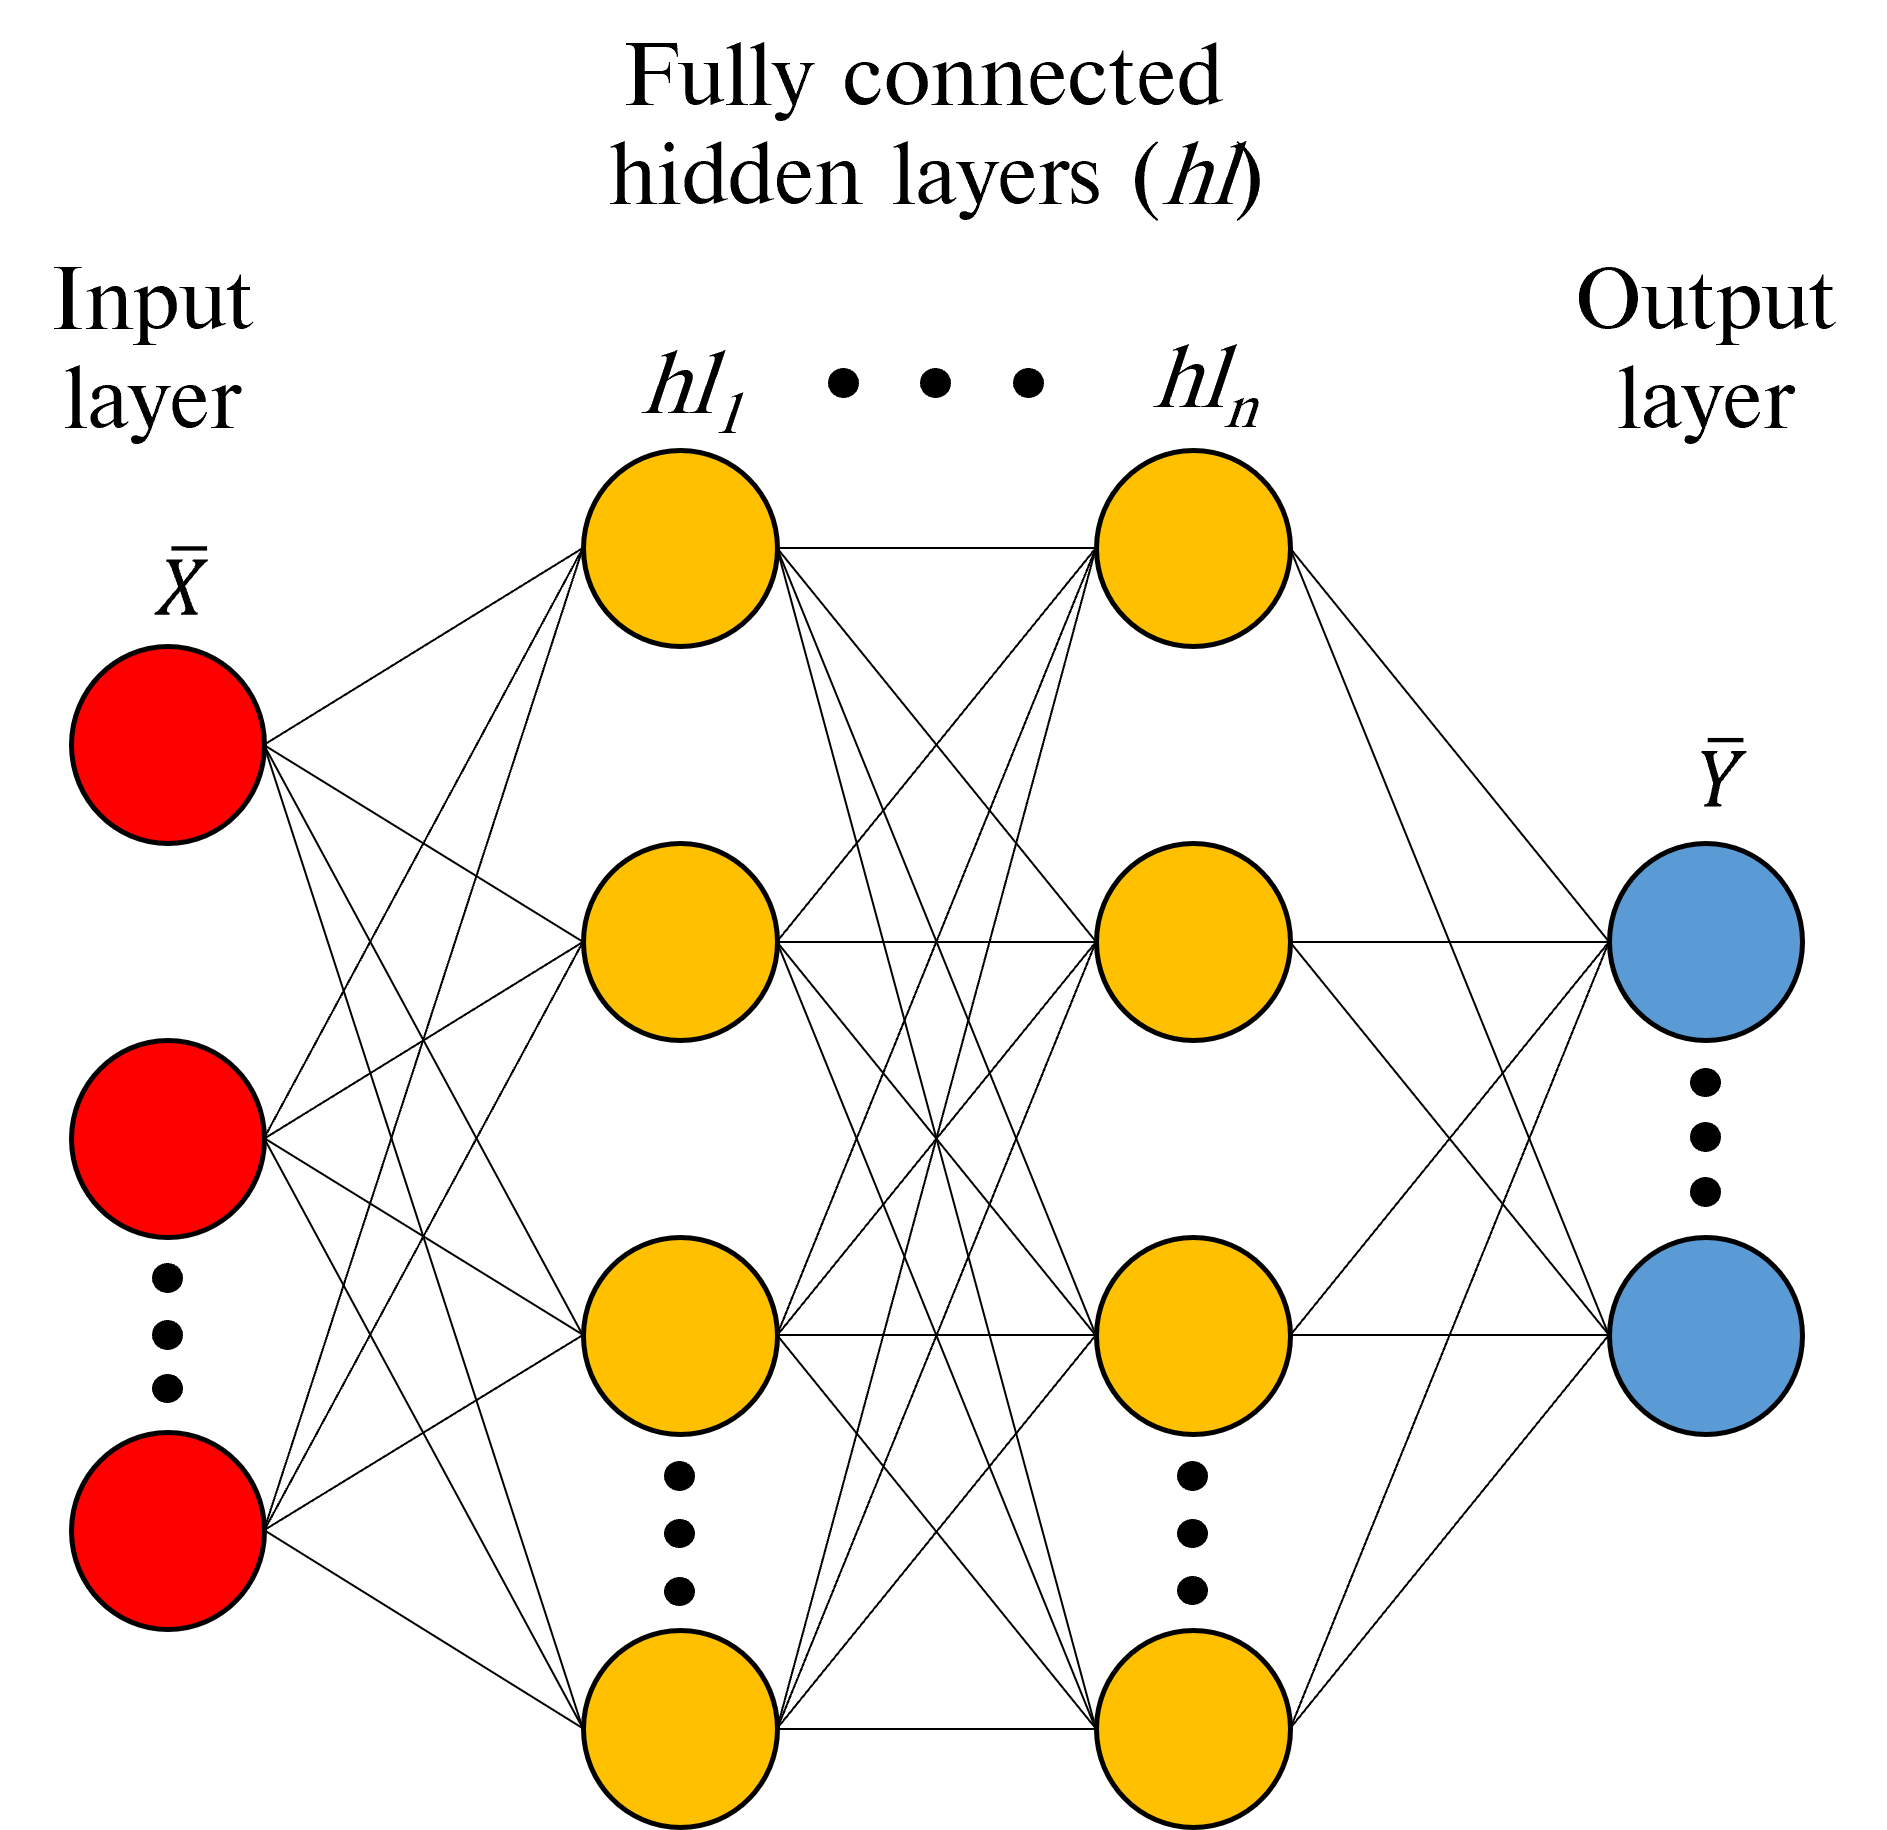
\includegraphics[scale=0.5]{ML_SCHEMATIC}
	  \caption{Traditional MLP schematic}\label{fig_mlp_schematic}
\end{figure}

To calculate the output values ($\hat{y_i}$) the forward propagation algorithm is utilized, which calculates the output for each layer and moves sequentially through the network till an output is determined. Each network layer output is calculated using two steps, the first being the calculation of the summed signal $\overline{z}_l$ and secondly the use of an activation function to generate the output signal $\overline{h}_l$. Equation \ref{eqn_summed_sig} highlights the first step, where $\overline{h}_{l-1}$ is the output signal from the previous layer.
\begin{equation}\label{eqn_summed_sig}
\overline{z}_l = \overline{h}_{l-1}\cdot\overline{w}_l+\overline{b}_l
\end{equation}

The result of the equation \ref{eqn_summed_sig} is subsequently passed to an activation function ($\overline{h}_l = \sigma_l(\overline{z}_l)$). There are various activation functions that can be utilized, such as linear, ReLu, Elu, and the hyperbolic-tangent \citep{goodfellow}, with the final layer activation function usually being linear for regression models. The current work makes use of ReLu and linear activation functions for the hidden layers. The ReLu and linear activation functions are shown in Equation \ref{eqn_act_func}.
\begin{equation}\label{eqn_act_func}
\begin{split}
&\overline{h}_l=\sigma_{ReLu}(\overline{z}_l) = \overline{z}_l =  
	\begin{cases}
	 \overline{h}_{l-1}\cdot\overline{w}_l+\overline{b}_l\,\, &if\,\,\,\, \overline{z}_l>0\\
	 0\,\, &if\,\,\,\, \overline{z}_l<0
	\end{cases}\\
&\overline{h}_l=\sigma_{linear}(\overline{z}_l) = \overline{z}_l = \overline{h}_{l-1}\cdot\overline{w}_l+\overline{b}_l
\end{split}
\end{equation}

When the forward propagation step is complete, the network weights and biases can be updated to minimize the cost function (refer to Equation \ref{eqn_lin_cost}) using the backward propagation method \ref{Rumelhart1986}. The methodology calculates the gradient of the cost function with respect to the weights and biases for each layer. Once the gradients have been calculated the weights and biases are updated using the gradient descent algorithm. The current work makes use of the Adam \cite{goodfellow} alternative to the gradient descent algorithm and is illustrated in Equation \ref{eqn_adam_algor}. Forward- and backward-propagation algorithms would be iteratively conducted until the cost function is reduced to below a desired threshold.

\begin{theorem} 
\begin{equation}\label{eqn_adam_algor} 
\begin{split}
&\overline{m}\leftarrow \beta_1\overline{m}+(1-\beta_1)\nabla_{\theta}J_{MSE}(\overline{\theta})\\
&\overline{s}\leftarrow \beta_1\overline{s}+(1-\beta_2)\nabla_{\theta}J_{MSE}(\overline{\theta})\otimes&\nabla_{\theta}J_{MSE}(\overline{\theta})\\
&\overline{m}\leftarrow\frac{\overline{m}}{1-\beta_1^t} \\
&\overline{s}\leftarrow\frac{\overline{s}}{1-\beta_2^t}\\
&\overline{\theta}\leftarrow\overline{\theta}-\eta\overline{m}\otimes(\sqrt{\overline{s}+\epsilon})^{-1}\\
\end{split}
\end{equation}
\end{theorem}

The variable $\bar{\theta}$, of Equation \ref{eqn_adam_algor}, represents the model parameters weights ($\bar{w}$) and biases ($\bar{b}$) for each layer. Scaling ($\bar{s}$) and momentum ($\bar{m}$) matrices are initialized to zero when beginning the training phase, $t$ is the iterative counter, $\beta_1$ and $\beta_2$ are the momentum and scaling decay hyper-parameters set to values of 0.9 and 0.999 respectively. Lastly $\epsilon$ is a smoothing term set to a value of $10^{-8}$.

\subsection{Mixture density networks (MDNs)}
Mixture density networks are fundamentally built from two components, that being an ANN and a mixture model, this allows for multi-modal predictions. The ANN can be a standard feed-forward MLP or a recurrent neural network (RNN), with RNNs traditionally being used in dynamic applications with at least one feedback loop \citep{Oko2015}. For this study the traditionally MLP is used.\\

MDNs are used to predict the parameters of a probability distribution ($P(\overline{X}\mid\overline{Y})$) allowing for non-Gaussian distributions to be modelled, thus making MDNs a probabilistic machine learning framework. MDNs estimate the conditional probability distribution as a mixture of Gaussian distributions where the mixing coefficients ($\overline{\pi}_k$) and component densities are flexible functions of the input data ($\overline{X}$). Equation \ref{eqn_cond_prob_func} illustrates the conditional probability function.
\begin{equation}\label{eqn_cond_prob_func}
P(\overline{X}\mid\overline{Y}) = \sum_{k=1}^K\pi_k(\overline{X})\cdot \mathbb{N}(\overline{Y}\mid \overline{\mu}_k(\overline{X}),\overline{\sigma}^2_k(\overline{X}))
\end{equation}
where $K$ represents the number of selected normal distributions, while $\overline{\mu}_k$ and $\overline{\sigma}^2_k$ are the predicted means and variances for each distribution $k$ given the input data $\overline{X}$ respectively.\\

A schematic of a simple ANN-MDN network is given in Figure \ref{fig_mdn_schematic}, highlighting the mixing coefficients, predicted means and deviations. It can is shown that modifications are made to the output layer by splitting the network output into three parts in order to calculate the $\overline{\pi}_k$, $\overline{\mu}_k$ and $\overline{\sigma}^2_k$ for each $k$ distribution. This enables the MDN network to learn the $P(\overline{X}\mid\overline{Y})$.\\

\begin{figure*}[h!]
	\centering
		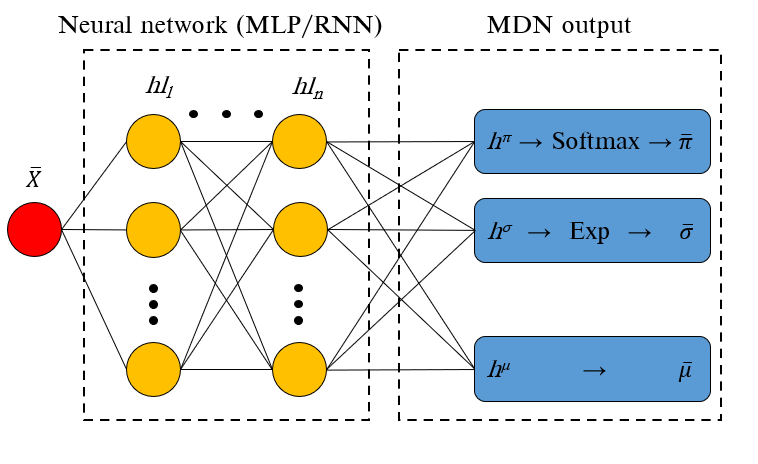
\includegraphics[scale=0.5]{MDN_SCHEMATIC}
	  \caption{Simple MDN network}\label{fig_mdn_schematic}
\end{figure*}

Bishop \cite{bishop1994} proposed the following restrictions for the mixing coefficients and variance components of the MDN output layer. Since the mixing coefficients contain the discrete probabilities of an output belonging to each $K$ normal distribution for all observations, the mixing coefficients must satisfy the constraints listed in Equation \ref{eqn_mix_coef_constraint}.
\begin{equation}\label{eqn_mix_coef_constraint}
\begin{split}
&\sum_{k=1}^K\overline{\pi}_k^n=1\\
&0\leq\overline{\pi}_k^n\leq1
\end{split}
\end{equation}
These constraints are met by using a Softmax function on the output of the hidden layer $h^{\pi}$. The mixing coefficient is calculated using Equation \ref{eqn_mix_coeff}.
\begin{equation}\label{eqn_mix_coeff}
\overline{\pi}_k^n(\overline{x}^n)=\frac{exp(h_k^{\pi,n})}{\sum_{k=1}^Kexp(h_k^{\pi,n})}
\end{equation}

Similarly a constraint is applied to the standard deviation values ensuring a positive value, this is achieved through the use of an exponential function being applied to the standard deviation leg of the MDN output layer, namely $h^{\sigma}$. Equations \ref{eqn_stddev} shows the imposed constraint for the standard deviation leg.\\
\begin{equation}\label{eqn_stddev}
\begin{split}
&(\overline{\sigma}^n_k(\overline{x}^n))^2\geq 0\\
&\sigma_k^n(\overline{x}^n)=exp(h_k^{\sigma,n})
\end{split}
\end{equation}

The MDN weights and biases are optimized by minimizing the negative log-likelihood for all observations in a batch, this is shown in Equation \ref{eqn_nll}.

\begin{equation}\label{eqn_nll}
\begin{split}
&J_{NLL}(\overline{Y},\overline{\pi},\overline{\sigma},\overline{\mu})=\\
&-\sum^N_{n=1}ln\left\{\sum^K_{k=1}\overline{\pi}_k(\overline{X}^n,\overline{\theta})\cdot \mathbb{N}(\overline{Y}^n\mid\overline{\mu}_k(\bar{X}^n,\bar{\theta}),\overline{\sigma}^2_k(\overline{X}^n,\overline{\theta})) \right\}
\end{split}
\end{equation}


\section{Data generation}
A steady-state multiphase non-thermal equilibrium CFD model was used to generate the target data, which was subsequently used for training/development of an appropriate surrogate model.

\subsection{CFD model setup}
The current study makes use of the commercial CFD software package ANSYS\textsuperscript{\textregistered} Fluent 2019 R3 to resolve the fluid flow, heat transfer and combustion processes for a 620$MW_e$ utility scale coal fired boiler. The computational domain is modelled on a symmetry plane half way through the depth of the boiler. Figure \ref{fig_cfd_geom_bc} highlights the computational domain and defines the important boundary conditions.\\ 

\begin{figure*}[h!]
	\centering
		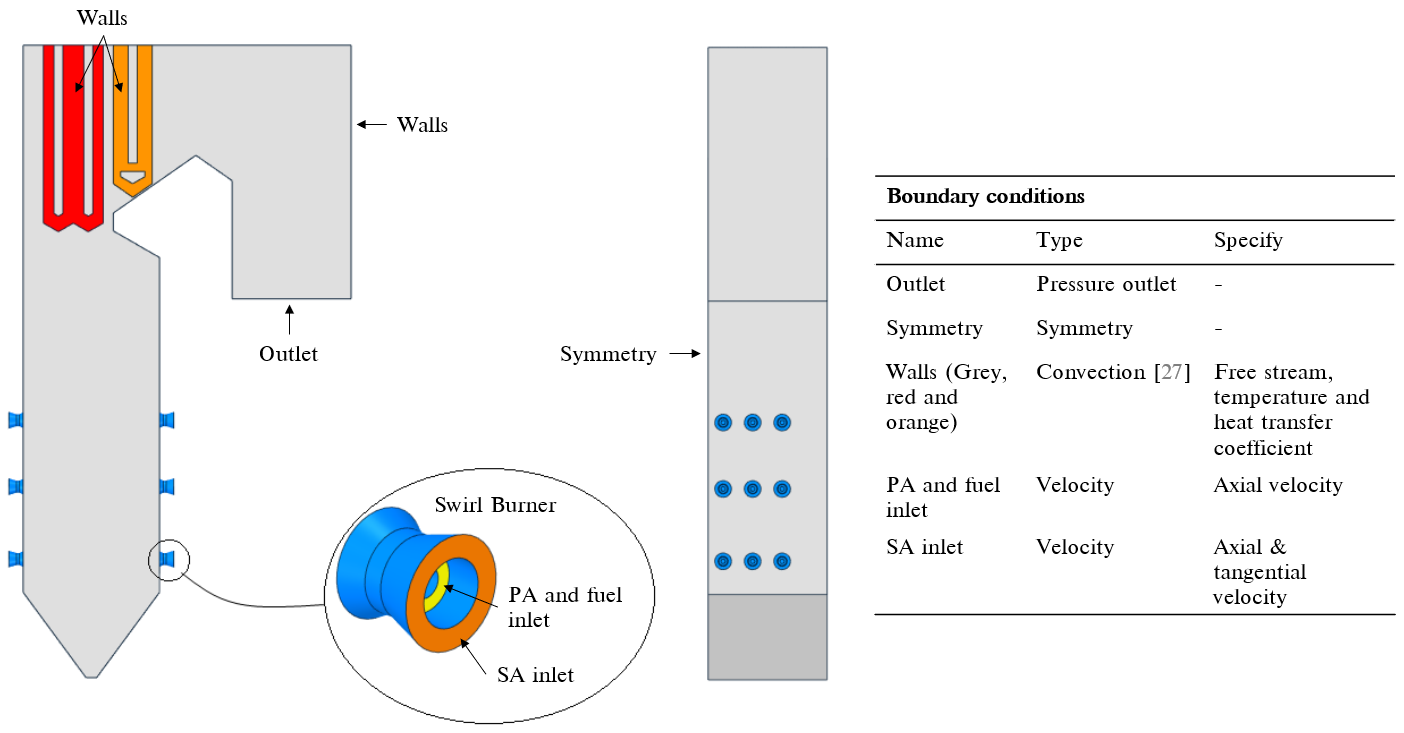
\includegraphics[scale=0.5]{CFD_GEOMETRY}S
	  \caption{CFD model geometry and boundary condition descriptions.}\label{fig_cfd_geom_bc}
\end{figure*}

The general conservation equations, which include, continuity, momentum, energy and species, were solved using a Eulerian approach. The subsequent equations are stated in Equation (\ref{eqn_cfd}).

\begin{flalign} \label{eqn_cfd}
&\frac{\partial}{\partial x_{i}}(\rho \bar{u}_{i})=S \nonumber &&\\
&\frac{\partial}{\partial x_{i}}(\rho_{eff} u_{i}u_{j})+\frac{\partial \overline{p}}{\partial x_{j}}= \nonumber&&\\
&\frac{\partial}{\partial x_{i}}\left[\mu\left\{\frac{\partial u_{j}}{\partial x_{i}}+\frac{\partial u_{i}}{\partial x_{j}}-\frac{2}{3}\delta_{ij}\frac{\partial u_{i}}{\partial x_{i}}\right\}\right]+\frac{\partial}{\partial x_{i}}(-\rho\overline{u_{i}^{'}u_{j}^{'}})+S_m \nonumber \nonumber &&\\
&\frac{\partial }{\partial x_{i}} (u_{i}[\rho E+p])=\frac{\partial }{\partial x_{j}}\left[\lambda\frac{\partial T_{g}}{\partial x_{j}}\right] +S_{h} &&\\
&\frac{\partial}{\partial x_{i}}(\rho u_{j}Y_{k})=-\frac{\partial}{\partial x_{j}}(\vec{J_{k}})+ \sum_r R_{j,r} + S_{k} \nonumber && 
\end{flalign}

The resolution of the Reynolds stress term found in the momentum equation, $-\rho\overline{u_{i}^{'}u_{j}^{'}}$, was approximated using the Boussineq equation \citep{Versteeg2007}. In the present study the realizable k-$\varepsilon$ turbulence model was utilized to address the turbulence closure problem, this model was selected for its applicability in modelling the effects of coal-fired swirl burners \citep{Modlinski2010}.\\

The P1 radiation model was used to resolve the radiative field in the domain. Particle transport was modelled using a multiphase approach, further details on the approach are provided in the validation study of Rawlins et al \citep{Rawlins2021}. The combustion follows a four step sequential process, beginning with the heating and evaporation of the moisture present in the fuel, followed by the devolatilization process where the volatiles are liberated from the solid particle, succeeded by the phenomena of char burnout, and finally the gas phase reactions would commence. The char oxidation reaction product species was set to that of carbon monoxide ($CO$). For the gas-phase reactions the turbulence-chemistry interaction was approximated using the eddy dissipation model (EDM). A summary of the combustion equations and constants are provided in Table \ref{tbl_combust}.\\

\begin{table*}[h!]
\caption{Summary of combustion models and constants used in the CFD model}\label{tbl_combust}
\begin{tabular*}{\tblwidth}{p{0.325\textwidth}p{0.35\textwidth}p{0.25\textwidth}}
\toprule
Model & Equation/s & Constant/s\\
\midrule
\multicolumn{3}{l}{\textit{Devolatilization}} \\ % Table header row
Single rate kinetic model &$\frac{dm_{vol}}{dt} = R_{vol}(m_{0,vol}-m_{vol})$,  & $A_{vol} = 2\times10^5 [s^{-1}]$, \\
& $R_{vol} = A_{vol}exp\left(\frac{E_{a,vol}}{RT_p}\right)$ & $ E_{a,vol} = 6.7\times10^7 [J/kmol]$ - \cite{Sheng2004} \\
\multicolumn{3}{l}{\textit{Char oxidation}} \\
Diffusion/kinetic - \citep{Baum1971} & $\frac{dm_{char}}{dt} = -A_p p_{O_{2}} \frac{R_{diff}R_c}{R_{diff} + R_c}$,  & $A_{c} = 0.0053 [kg/m^2sPa]$, \\
& $R_{c} = A_{c}exp\left(\frac{E_{a,c}}{RT_p}\right)$,  & $E_{a,c} = 8.37\times10^7 [J/kmol]$ - \cite{Sheng2004} \\
& $R_{diff} = \frac{5\times10^{-12}}{d_p} \left(\frac{T_g+T_p}{2}\right)^{0.75}$&\\
\multicolumn{3}{l}{\textit{Gaseous reactions of volatiles and $CO$}} \\
Eddy dissipation model - \cite{Ansys} & $R_{k,r,P} =\vartheta_{k,r}M_{w,k}AB\rho\frac{\varepsilon}{k}min\left(\frac{\sum_{p} Y_p}{\sum_{j}\vartheta_{j,r}M_{w,j}}\right)$, $R_{k,r,R} =\vartheta_{k,r}M_{w,k}A\rho\frac{\varepsilon}{k}min\left(\frac{Y_R}{\varepsilon_{R,r}M_{w,R}}\right)$ & $A=4.0$, $B=0.5$\\
\bottomrule
\end{tabular*}
\end{table*}

The simulations were solved using the SIMPLE pressure–velocity coupling scheme. The pressure term was discretized using the PRESTO! scheme. Momentum, species and energy equations were discretized using the second-order upwind scheme and the turbulent kinetic energy and dissipation rate using the first-order upwind scheme. The numerical mesh was generated using quadrilateral elements consisting of 6 million cells.  The convergence criteria for the simulation model was set to $1\times10^{-3}$ for the continuity equation, $1\times10^{-4}$ for the velocity equations, $1\times10^{-6}$ for the remaining transport equations, and $1\times10^{-4}$ for monitored key parameters.

\subsection{Simulated dataset}
As previously mentioned the aim this study is to illustrate the use of a data-driven surrogate model, integrated with a 1D process model, to predict the heat loads to the various heat exchanging components, the flue-gas composition and exit gas temperatures for a utility scale boiler using various high-level inputs. The inputs include the the following, the excess air ratio per burner, the total mill flowrate for the six mills in operation, the average steam temperatures for the platen and final superheaters, the fouling resistance for the platen and final superheaters, the composition of ash and moisture of the fuel and the gross calorific value of the fuel. Thus the input field has a dimensionality of $d_{inputs}=14$.\\

A design of experiments (DOE) was conducted to generate a set of 180 simulation cases to obtain a representative set of results. The various model input ranges used in the DOE are given in Table \ref{tbl_doe}. The ranges where selected to cover a wide range of operational loads with maximum continuous ratings (MCR) between 100\% and 30\%. A total of 27 output target values ($d_{targets}$) are realised for each CFD simulation case. Due to the quasi-steady nature of the CFD simulations, output target values for were taken every 50 iterations for the last 2500 iterations for a converged CFD simulation. This results in each CFD simulation case having a data solution matrix size of ($\bar{Y}\in50\times27$).\\

The DOE matrix was populated using the Latin Hypercube Sampling (LHS) method provided in the Python $pyDOE$ library. Once the CFD simulations achieved convergence, the target data, comprising of the discretized heat loads to the furnace, platen and final SHs, the exit flue-gas temperatures and combustion characteristics, was stored for each case. The target dataset was split with 80\% being used for training purposes and the remainder for testing. To reduce the training time of the neural networks a min-max normalization was utilized scaling all the dataset entries to values between $0\rightarrow1$.\\

\begin{table*}[h!]
\caption{Design of experiments input ranges for  simulations}\label{tbl_doe}
\begin{tabular*}{\tblwidth}{p{0.5\textwidth}p{0.15\textwidth}p{0.15\textwidth}p{0.15\textwidth}}
\toprule
 Input variables& Min& Max& Units \\ % Table header row
\midrule
 Total fuel flow rate for mills 1 to 6 & 39.5 & 120.2 & $kg/s$ \\
 Fuel proximate analysis moisture mass fraction, $Y_{H_2O}$ & 0.025 & 0.085 & $kg/kg$ \\
 Fuel proximate analysis ash mass fraction, $Y_{ash}$  & 0.259 & 0.559 & $kg/kg$ \\
 Platen SH fouling thermal resistance, $R_{platen}$  & 0.004 & 0.007 & $m^2K/W$ \\
 Final SH fouling thermal resistance, $R_{final}$  &0.01 & 0.017 & $m^2K/W$ \\
\midrule
Dependent variables& \multicolumn{2}{l}{Function of}& Units\\
\midrule
Higher heating value&\multicolumn{2}{l}{Fuel constituents $Y_{H_2O}$ and $Y_{ash}$}&$J/kg$\\
Excess air & \multicolumn{2}{l}{Total fuel flow rate for mills} & $\%$\\
Platen SH internal steam temperature& \multicolumn{2}{l}{$R_{platen}$} & $K$\\
Final SH internal steam temperature& \multicolumn{2}{l}{$R_{final}$} & $K$\\
\bottomrule
\end{tabular*}
\end{table*}
\section{Model development}
The present work makes use of two types of machine learning models, namely a standard artificial neural network (ANN/MLP) and a mixture density designated model connected to a standard ANN (MDN-ANN). The following section will discuss the hyper parameter tuning and final selected model configuration. The programming language Python 3.7.8 and the Tensorflow machine learning libraries were utilized in the present study. 
\subsection{Model configuration}
The goal of the final machine learning configuration is to be able to predict the heat load distributions to the furnace, platen SH and final SH walls, the combustion characteristics and flue-gas temperatures at the exit, using the high level inputs given in Table \ref{tbl_doe}.\\

The outputs for the MLP will consist of $y=50\times180=9000$ outputs. Thus, for a data batch size, $m_b$, the output tensor for the MLP model will be $\hat{Y}\in \mathbb{R}^{m_b\times y\times 27}$ since $d_{targets}=27$. However, the MDN-ANN models output data will consist of three parts, namely; the mixing coefficients tensor of shape  $\overline{\pi}\in \mathbb{R}^{m_b \times y\times K}$, the output standard deviation tensor of shape $\overline{\sigma}\in \mathbb{R}^{K\times m_b\times y\times 27}$ and the predicted means of tensor shape $\overline{\mu}\in \mathbb{R}^{K\times m_b\times y\times 27}$. The input data fed into both the MLP and MDN-ANN will have shape $\overline{X}\in \mathbb{R}^{m_b\times d_{inputs}}$. The input features will be varied based on the DOE, to account for burner mill biassing, fuel quality and SH heating component fouling.\\
\subsection{Hyper-parameter tuning \& final model selection}
Table \ref{tbl_tuning} highlights the hyper-parameter search spaces for both the ANN and ANN-MDN model. The ANN-MDN has an added parameter namely the number of additional distributions the ANN-MDN would fit to the output data. \\

\begin{table*}[h!]
\caption{Hyper-parameter search space for fully connected NN and MDN models}\label{tbl_tuning}
\begin{tabular*}{\tblwidth}{p{0.5\textwidth}p{0.24\textwidth}p{0.24\textwidth}}
\toprule
 Parameter& NN search space & MDN search space \\ % Table header row
\midrule
 Number of distributions & - & 1,2,3,4  \\
 Number of layers & 2,3,4 & 2,3,4\\
 Number of neurons per layer & 10, 40, 80, 100  & 10, 40, 80, 100\\
 Learning rates & 1e-3, 1e-4, 1e-5, 1e-6 &  1e-3, 1e-4, 1e-5, 1e-6   \\
 Mini batch sizes  &32, 64, 128, 256 &32, 64, 128, 256  \\
\bottomrule
\end{tabular*}
\end{table*}


The hyper-parameter search was conducted in a sequential manner with the number of layers and neurons per layer being the initial step, after which the learning rates were varied, followed by the batch sizes. The ANN-MDN hyper-parameter tuning was conducted in a similar manner only that an additional step is required to establish the best amount of distributions.

\begin{table*}[h!]
\caption{ANN model selection results}\label{tbl_tuning}
\begin{tabular*}{\tblwidth}{p{0.5\textwidth}p{0.24\textwidth}p{0.24\textwidth}}
\toprule
 Parameter& NN search space & MDN search space \\ % Table header row
\midrule
 Number of distributions & - & 2,3,4  \\
 Number of layers & 2,3,4 & 2,3,4\\
 Number of neurons per layer & 10, 40, 80, 100  & 10, 40, 80, 100\\
 Learning rates & 1e-3, 1e-4, 1e-5 &  1e-3, 1e-4, 1e-5   \\
 Mini batch sizes  & 16, 32, 64 & 16, 32, 64  \\
\bottomrule
\end{tabular*}
\end{table*}
\subsection{Process model integration}
Th validation and the subsequent case-studies of Section \ref{sec_results_diss}, make use of an integrated surrogate and network based-process model. The process model is used to capture the thermodynamic response of the water/steam side of the utility boiler under investigation, the the developed data-driven surrogate model providing the gas-side thermal predictions.\\

A C\# script is used to access the Python API available in the process modelling software, Flownex SE\textsuperscript{\textregistered} 2021. This allows for predictions to be made using the trained MDN-ANN model (surrogate model). The most probable predictions are retrieved using the script and transferred to the respective process model components as inputs. A schematic of the surrogate and process models integration is provided in Figure \ref{fig_int_model}.
\begin{figure*}[h!]
	\centering
		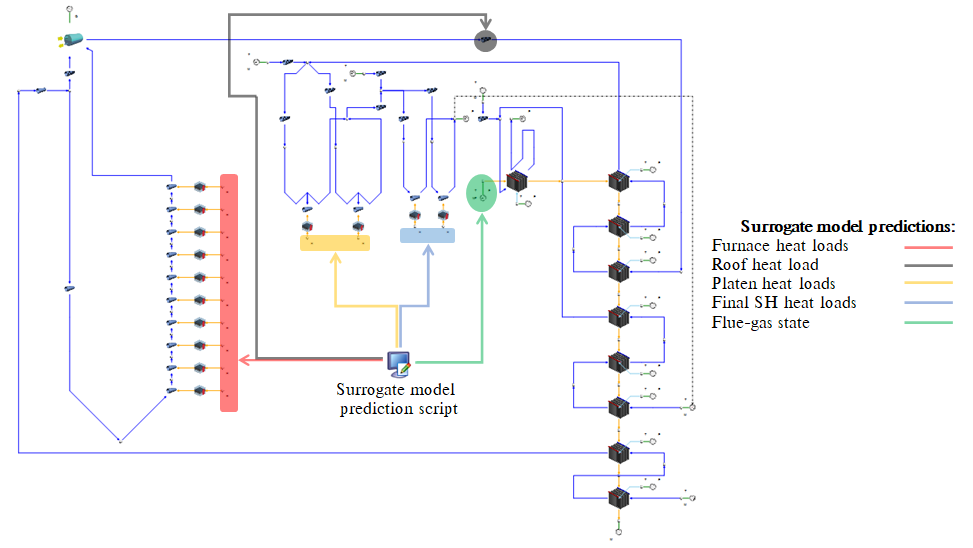
\includegraphics[scale=0.65]{INTEGRATED_MODEL}S
	  \caption{Schematic of integrated surrogate and network based process model}\label{fig_int_model}
\end{figure*}
fhhf


\section{Results and discussion}\label{sec_results_diss}
A illustrated in the previous section the MDN-ANN model is selected model used for the subsequent validation and fuel quality case studies.

\subsection{Multiple load validation}




Measured plant data for a 100\%, 81\% and 60\% MCR load ratings was made available and is to be used compare the accuracy of the integrated model.
\subsection{Utility boiler response to poor fuel combustion}
The fuel quality is an important factor when determining the 
Fuels with total moisture contents exceeding 
The following results illustrate the effects poor quality fuel has on the case studies boiler operational. The study made use of the developed surrogate model to investigate the steady state operation of the boiler burning poor quality coal.  
In this section the results of a study conducted  
\section{Conclusion}

The present work has shown it is possible
% To print the credit authorship contribution details
\printcredits

%% Loading bibliography style file
%\bibliographystyle{model1-num-names}
\bibliographystyle{cas-model2-names}
\newpage
% Loading bibliography database
\bibliography{ML_paper}

% Biography
\bio{}
% Here goes the biography details.
\endbio

%$\bio{pic1}
% Here goes the biography details.
%\endbio

\end{document}

